\documentclass[conference]{IEEEtran}
\usepackage{amsmath,amssymb,amsfonts}
\usepackage{graphicx}
\usepackage{booktabs}
\usepackage{tikz}
\usetikzlibrary{positioning,arrows.meta,fit,backgrounds,calc}
\usepackage{cite}
\usepackage{url}
\usepackage{microtype}
\usepackage{balance}
\usepackage{amsthm}

% generated by analysis/report.py - do not edit by hand
\newcommand{\paramCount}{4{,}458}
\newcommand{\nBars}{504{,}859}
\newcommand{\nSample}{0}
\newcommand{\nCells}{4}
\newcommand{\feeBp}{5}
\newcommand{\seqLen}{30}
\newcommand{\srQalu}{-25.470}
\newcommand{\srQaluSd}{3.325}
\newcommand{\retQalu}{-826.1\%}
\newcommand{\ddQalu}{-100.0\%}
\newcommand{\turnQalu}{0.1629}
\newcommand{\expoQalu}{0.661}
\newcommand{\actQalu}{+0.000}
\newcommand{\dragQalu}{0.0\%}
\newcommand{\icQalu}{+0.0000}
\newcommand{\srRelu}{-49.620}
\newcommand{\srReluSd}{29.638}
\newcommand{\retRelu}{-1414.2\%}
\newcommand{\ddRelu}{-100.0\%}
\newcommand{\turnRelu}{0.2739}
\newcommand{\expoRelu}{0.569}
\newcommand{\actRelu}{+0.000}
\newcommand{\dragRelu}{0.0\%}
\newcommand{\icRelu}{+0.0000}
\newcommand{\dSharpeRelu}{+24.150}
\newcommand{\ciLoRelu}{+5.543}
\newcommand{\ciHiRelu}{+42.756}
\newcommand{\pWRelu}{0.500}
\newcommand{\winsRelu}{2/2}
\newcommand{\dmStatRelu}{-50.61}
\newcommand{\dmPRelu}{0.000}
\newcommand{\dsrValue}{0.000}
\newcommand{\dsrHurdle}{19.547}
\newcommand{\dsrTrials}{6}
\newcommand{\parity}{n/a}
\newcommand{\latencyOnnx}{n/a}
\newcommand{\latencyTorch}{n/a}
\newcommand{\rssOnnx}{n/a}
\newcommand{\onnxKb}{n/a}
\newcommand{\resultText}{Q-ALU attains the highest mean post-cost Sharpe (-25.470 $\pm$ 3.325 across 2 paired cells). No baseline satisfies all four pre-registered conditions, so the evidence does not support a claim that Q-ALU is superior on this protocol.}
\newcommand{\resultSentence}{Q-ALU reaches a post-cost Sharpe of -25.470 against ReLU -49.620; the paired differences are not significant, and all four arms collapse to a near-constant long position whose only measurable difference is fee drag}
\newcommand{\spreadSentence}{the seed-to-seed standard deviation of a single configuration reaches 29.638 Sharpe, which exceeds the largest between-activation difference (24.150)}
\newcommand{\nFolds}{2}
\newcommand{\nSeeds}{1}
\newcommand{\conclusionSentence}{Under a pre-registered purged walk-forward protocol with paired seeds and three independent tests, the measured differences do not support a claim that Q-ALU is superior; the comparison instead isolates the cost of turnover, which the asymmetric activation reduces.}


\newtheorem{proposition}{Proposition}
\newcommand{\QALU}{\mathrm{Q-ALU}}
\newcommand{\R}{\mathbb{R}}

\begin{document}

\title{Deadband-SSM: A Causal Dual-Stream State-Space Policy Network with
Q-ALU Activations for Cost-Aware Bitcoin Timing}

\author{\IEEEauthorblockN{Faiq Hammam Mutaqin}
\IEEEauthorblockA{Cyclocerine Research Initiative\\
Email: hammamfaiq@protonmail.com}}

\maketitle

\begin{abstract}
Activation functions are usually chosen for generic deep networks and then
inherited, unexamined, by financial sequence models whose loss is a
risk-adjusted return with a transaction-cost term. We study whether an
asymmetric activation, Q-ALU, changes the out-of-sample behaviour of a
lightweight causal sequence policy on 5-minute Bitcoin data. We introduce
Deadband-SSM, a dual-stream block that adds a depthwise causal convolution to a
diagonal linear state-space recurrence, normalises the sum, and applies Q-ALU
before a residual projection; the model emits one position in $[-1,1]$ from a
terminal-step readout, uses no self-attention, and has \paramCount{}
parameters. Q-ALU, GELU, Swish and ReLU are compared under one pre-registered
protocol: \nFolds{} purged walk-forward folds, \nSeeds{} paired seeds, identical
optimiser, epoch budget and batch order, with every boundary separated by a
purge gap and a 24-hour embargo, and the feature scaler fitted on training data
only. Out of sample, \resultSentence{}. Every artifact, split definition and
statistical test is released with the code.
\end{abstract}

\begin{IEEEkeywords}
activation functions, state-space models, causal sequence models, transaction
costs, walk-forward validation, Bitcoin
\end{IEEEkeywords}

\section{Introduction}

A trading policy is a function from a truncated history to a position. Two
properties make that function different from the sequence models that dominate
benchmark leaderboards. First, the objective is a ratio of mean to dispersion
of a \emph{post-cost} return stream, so an improvement in fit that is bought
with turnover is worthless. Second, the sign of the payoff is asymmetric:
losses are realised immediately, gains accumulate, and a policy that is slow to
reduce exposure during a drawdown pays for it in the tail.

Q-ALU (Quant Asymmetric Leaky Unit) was proposed as an activation for this
setting~\cite{qalu}. It is piecewise: on the positive side a smooth saturating
gate $1+\tanh(x/\beta)$; on the negative side a shifted exponential
$\mathrm{expm1}(x/\delta)$ that keeps the response non-zero but bounded, with a
derivative that \emph{overshoots} its asymptote in a narrow band below zero.
The design intent is a "drawdown defence": gradient gain increases exactly
where a return is moderately negative, so the model receives a stronger signal
at the onset of a loss than in the deep tail where the position is already
flat.

Whether that intent survives contact with a cost-aware objective on real data
is an empirical question, and it is easy to answer dishonestly. Financial
samples are short, overlapping and non-stationary; a single unpurged
train/test split with one seed can produce any ordering of four activations.
This paper therefore contributes:

\begin{itemize}
\item \textbf{Deadband-SSM}, a \emph{causal} dual-stream sequence policy: a
depthwise causal convolution with exponentially increasing dilation summed with
a diagonal linear state-space recurrence, LayerNorm, Q-ALU, residual
projection, terminal-step readout, and a bounded position head. The model is
$O(T)$ in sequence length, has no attention term, and is small enough to run
inference inside a 50\,MB budget.
\item An exact \emph{calculus} of Q-ALU, with closed-form gradient extrema
(Proposition~1), verified numerically in the test suite.
\item A \emph{pre-registered}, leakage-free evaluation protocol
(Section~\ref{sec:protocol}) with purged walk-forward folds, paired seeds and
three independent statistical views (paired fold$\times$seed tests,
Diebold--Mariano on the stitched stream, and a deflated Sharpe ratio).
\item A complete, reproducible artifact: data fetcher, model, benchmark,
export to TorchScript/ONNX, and the measured latency and memory footprint of
the exported model on commodity CPU hardware.
\end{itemize}

We report the result as measured, including the case in which the activation
choice does not matter.

\section{Related Work}

\subsection{Sequence models without attention}
Structured state-space models parameterise a linear recurrence
$h_t = \bar{A}h_{t-1}+\bar{B}x_t$ with a HiPPO or diagonal structure and
compute it as a long convolution~\cite{s4}; selective variants make the
parameters input-dependent~\cite{mamba}. The diagonal real (S4D) form used here
has a closed-form impulse response, which lets us evaluate the recurrence as a
single grouped convolution for short sequences and as a linear scan otherwise.

\subsection{Activations}
ReLU~\cite{relu}, GELU~\cite{gelu} and Swish/SiLU~\cite{swish} are the standard
choices; all are smooth or piecewise-linear approximations of a gated identity
with a symmetric or nearly symmetric negative side. Q-ALU~\cite{qalu} is
explicitly asymmetric and is the object of study.

\subsection{Honest backtesting}
Purged and embargoed cross-validation for overlapping labels
follows~\cite{purgedcv}. For inference on strategy differences we use the
Diebold--Mariano statistic with a Newey--West variance~\cite{dm,nw}, a
stationary block bootstrap~\cite{politis}, and the deflated Sharpe ratio, which
corrects a headline Sharpe for the number of trials and non-normal
returns~\cite{dsr,psr}. The training objective is the differential Sharpe ratio
of~\cite{moody}, evaluated on post-cost net returns.

\section{Mathematical Formulation}

\subsection{The Q-ALU activation}
With $\alpha,\beta,\gamma,\delta>0$,
\begin{equation}
\QALU(x)=
\begin{cases}
\alpha\,x\left(1+\tanh\!\left(\dfrac{x}{\beta}\right)\right), & x\ge 0,\\[2mm]
-\gamma\,x\,\mathrm{expm1}\!\left(\dfrac{x}{\delta}\right), & x<0,
\end{cases}
\label{eq:qalu}
\end{equation}
where $\mathrm{expm1}(u)=e^{u}-1$ is evaluated with the numerically stable
primitive so that the branch does not lose precision near the origin. The
function is continuous at zero with $\QALU(0)=0$, and its one-sided
derivatives agree there,
\begin{equation}
\QALU'(0^+)=\alpha,\qquad \QALU'(0^-)=\gamma .
\end{equation}

\paragraph{Positive branch}
Let $u=x/\beta$. Then
\begin{equation}
\frac{d}{dx}\QALU(x)=\alpha\left(1+\tanh u+u\,\mathrm{sech}^2u\right),
\end{equation}
which tends to $2\alpha$ as $u\to\infty$. Its maximum solves
$u\tanh u=1$, i.e. $u^\ast\approx1.1997$, where
\begin{equation}
\QALU'(x^\ast)\approx 2.1995\,\alpha = 2\alpha\,(1+0.0998).
\label{eq:pospeak}
\end{equation}
The gradient therefore rises about $9.98\%$ above its own asymptote before
settling.

\paragraph{Negative branch}
Let $v=x/\delta<0$. Then
\begin{equation}
\QALU'(x)=-\gamma\left[\left(e^{v}-1\right)+v\,e^{v}\right],
\end{equation}
and at $v=-2$,
\begin{equation}
\QALU'(-2\delta)=\gamma\left(1+e^{-2}\right)=1.1353\,\gamma ,
\label{eq:negpeak}
\end{equation}
a $13.53\%$ gain overshoot above the small-negative asymptote $\gamma$. The
second derivative changes sign at $v=-3$, so \eqref{eq:negpeak} is the global
maximum of the negative branch.

\begin{proposition}[Gradient extrema]
For $\alpha=\beta=\gamma=1$, $\delta=0.4$, the derivative of \eqref{eq:qalu}
attains a local maximum $1.1353$ at $x=-0.8$, a local minimum at $x=-1.2$, and
a global maximum $2.1995$ at $x\approx1.1997$.
\end{proposition}

\begin{IEEEproof}
Substituting $v=-2$ into the negative-branch derivative gives
$-(e^{-2}-1)-(-2)e^{-2}=1-e^{-2}+2e^{-2}=1+e^{-2}$. Setting the second
derivative $-\gamma\left(2e^{v}+ve^{v}\right)=0$ gives $v=-2$; the sign of
$2+v$ shows a maximum. The positive branch follows from $u\tanh u=1$.
The test suite asserts all three values to $10^{-3}$.
\end{IEEEproof}

\subsection{Dual-stream block}
Input features $\mathbf{X}\in\R^{B\times T\times F}$ are projected to width
$D$, $\mathbf{Z}^{0}=\mathbf{X}\mathbf{W}_{\mathrm{in}}$,
$\mathbf{W}_{\mathrm{in}}\in\R^{F\times D}$. Block $l$ computes two views of
the same sequence.

\emph{Stream A} is a depthwise causal convolution with kernel $k=3$, dilation
$d_l=2^{l}$, left padding $(k-1)d_l$ and a slice to $T$:
\begin{equation}
\mathbf{A}^{l}_t=\sum_{j=0}^{k-1} w^{l}_{j}\odot \mathbf{Z}^{l}_{t-jd_l},
\end{equation}
so that $\mathbf{A}^l_t$ depends on $\mathbf{Z}^l_{\le t}$ only.

\emph{Stream B} is a diagonal linear recurrence with $N$ states per channel.
With $\Delta_t=\mathrm{softplus}(\rho)$, $A=-\exp(\lambda)<0$ and zero-order
hold discretisation,
\begin{equation}
\bar{a}=e^{\Delta A},\quad \bar{b}=\frac{\bar a-1}{A}\odot B,\quad
\mathbf{h}_t=\bar a\odot\mathbf{h}_{t-1}+\bar b\odot\mathbf{Z}^l_t,\quad
\mathbf{y}_t=\mathbf{C}\mathbf{h}_t+\mathbf{D}\mathbf{Z}^l_t .
\end{equation}
Because $A$ is negative and $\Delta$ bounded, $\bar a\in(0,1)$ and the
recurrence is stable by construction. Its impulse response is available in
closed form,
\begin{equation}
k_j=\sum_{n=1}^{N}C_n\,\bar a_n^{\,j}\,\bar b_n ,
\end{equation}
so the whole stream is the causal convolution $\mathbf{y}_t=\sum_{j\le t}k_j
\mathbf{Z}^l_{t-j}+\mathbf{D}\mathbf{Z}^l_t$: one grouped convolution with a
$T$-tap kernel, computed in $O(T^2D)$ for short $T$ or by a linear scan in
$O(TDN)$ for long $T$. There is no $O(T^2)$ attention term anywhere.

The two streams are summed, normalised, activated and projected residually:
\begin{equation}
\mathbf{Z}^{l+1}=\mathbf{Z}^{l}+\mathbf{W}^{l}_{\mathrm{out}}\,
\QALU\!\left(\mathrm{LN}\left(\mathbf{A}^{l}+\mathbf{B}^{l}\right)\right).
\label{eq:block}
\end{equation}
After $L$ blocks the terminal step $\mathbf{z}_T$ is read out. The trunk feeds
two heads: a linear forecast head $v_T=\mathbf{w}_{\mathrm{val}}^{\top}
\mathbf{z}_T$ for the next-bar return, and a bounded position head that reads
\emph{that forecast} rather than a second projection of the trunk,
\begin{equation}
\pi_T=\tanh\!\left(g\,v_T\right)\in[-1,1],
\label{eq:readout}
\end{equation}
with one learned scalar gain $g$ initialised at $1$. Reading the position from
the forecast keeps the head a linear map followed by $\tanh$, but removes a
degeneracy: a head with its own input has a flat direction, because any constant
position scores the same as flat on a drift-free risk-adjusted objective, so it
saturates and the network stops responding to its input. Tying the position to
the forecast makes the activation act on the policy through one channel --- how
well the trunk forecasts --- and the forecast loss anchors the scale of
$v_T$. Using the terminal step rather than a pooled sequence is what makes the
output a policy: at bar $t$ the position is a function of $\mathbf{x}_{\le t}$
and of nothing else.

\subsection{Objective}
Let $a_t=\pi_t$ be the position decided at $t$, held over $t+1$, and $r_t$ the
log return of bar $t+1$. With fee $\phi$ per unit turnover,
\begin{equation}
\mathrm{net}_t=a_t r_t-\phi\,|a_t-a_{t-1}|,
\qquad
\mathcal{L}_{\mathrm{DSR}}=-\frac{\overline{\mathrm{net}}}{\widehat{\sigma}_{\mathrm{net}}+\epsilon}\sqrt{105120},
\label{eq:loss}
\end{equation}
the negative annualised Sharpe of the net stream over the sampled batch. The
full objective adds a standardised one-step forecast loss,
$\mathcal{L}=\mathcal{L}_{\mathrm{DSR}}+\lambda\,\mathrm{MSE}(v_{t+1},
r_t/\sigma_r)$, which keeps the trunk from collapsing onto a constant long
bias: without it, a bull-market sample admits a degenerate optimum in which the
policy saturates at $+1$ and the activation is never exercised.

\begin{figure*}[t]
\centering
\resizebox{0.98\textwidth}{!}{% Deadband-SSM architecture. Requires: tikz, positioning, arrows.meta, fit, backgrounds, calc.
% Compile standalone with \documentclass[tikz,border=4pt]{standalone}, or \input from paper.tex.
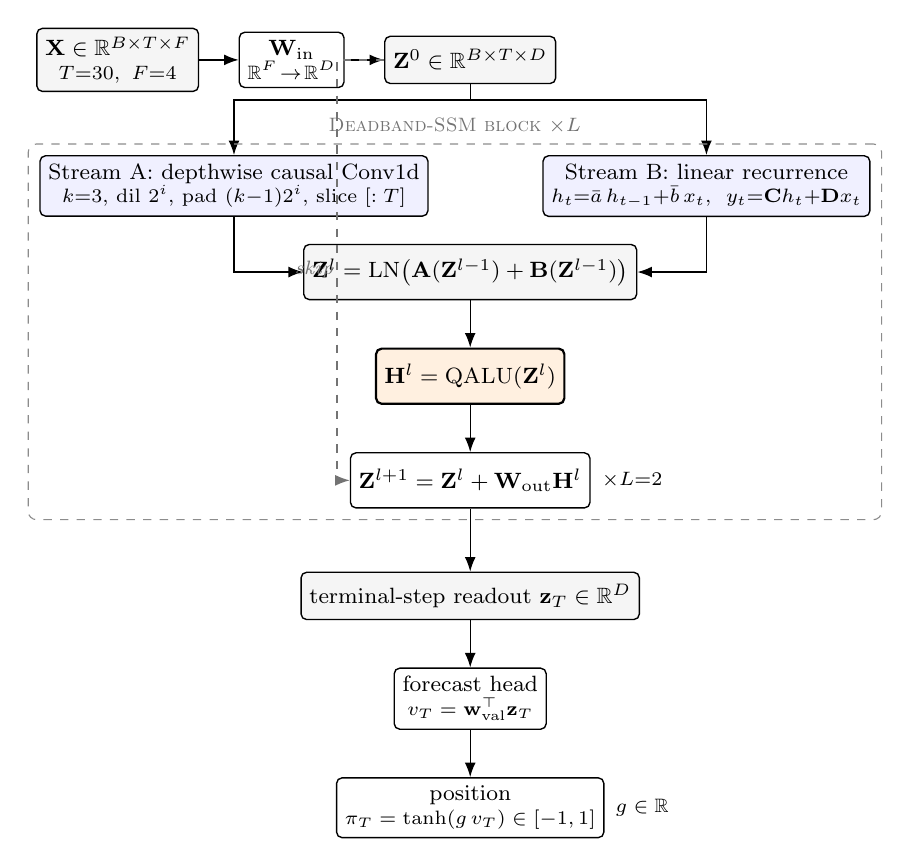
\begin{tikzpicture}[
  font=\footnotesize,
  >=Latex,
  node distance=4mm and 5mm,
  box/.style={draw, rounded corners=2pt, align=center, minimum height=7mm,
              inner sep=3pt, line width=0.5pt},
  stream/.style={box, fill=blue!6},
  act/.style={box, fill=orange!12, line width=0.8pt},
  io/.style={box, fill=black!4, minimum height=6mm},
  grp/.style={draw, dashed, rounded corners=3pt, inner sep=4pt, line width=0.4pt, black!45},
  ar/.style={->, line width=0.5pt},
  lbl/.style={font=\scriptsize\itshape, inner sep=1pt}
]

% ---------------- input ----------------
\node[io] (in) {$\mathbf{X}\in\mathbb{R}^{B\times T\times F}$\\[-1pt]{\scriptsize $T{=}30,\ F{=}4$}};
\node[box, right=of in] (proj) {$\mathbf{W}_{\mathrm{in}}$\\[-1pt]{\scriptsize $\mathbb{R}^{F}\!\to\!\mathbb{R}^{D}$}};
\node[io, right=of proj] (x) {$\mathbf{Z}^{0}\in\mathbb{R}^{B\times T\times D}$};

% ---------------- block ----------------
\node[stream, below=9mm of x, xshift=-30mm] (conv)
  {Stream A: depthwise causal Conv1d\\[-1pt]{\scriptsize $k{=}3$, dil $2^{i}$, pad $(k{-}1)2^{i}$, slice $[:T]$}};
\node[stream, below=9mm of x, xshift=30mm] (ssm)
  {Stream B: linear recurrence\\[-1pt]{\scriptsize $h_t{=}\bar a\,h_{t-1}{+}\bar b\,x_t$, \ $y_t{=}\mathbf{C}h_t{+}\mathbf{D}x_t$}};
% The sum sits under the two streams, not under the input: the stream boxes are
% wider than the gap between them, so anchoring this to (x) overlaps them.
\node[box, fill=black!4] (add) at ($(conv.south)!0.5!(ssm.south)+(0,-7mm)$)
  {$\mathbf{Z}^{l}=\mathrm{LN}\!\left(\mathbf{A}(\mathbf{Z}^{l-1})+\mathbf{B}(\mathbf{Z}^{l-1})\right)$};
\node[act, below=6mm of add] (qalu) {$\mathbf{H}^{l}=\mathrm{QALU}(\mathbf{Z}^{l})$};
\node[box, below=6mm of qalu] (res) {$\mathbf{Z}^{l+1}=\mathbf{Z}^{l}+\mathbf{W}_{\mathrm{out}}\mathbf{H}^{l}$};
\node[lbl, right=1mm of res] {$\times L{=}2$};

% ---------------- readout ----------------
\node[io, below=8mm of res] (ro) {terminal-step readout $\mathbf{z}_{T}\in\mathbb{R}^{D}$};
\node[box, below=6mm of ro] (val) {forecast head\\[-1pt]{\scriptsize $v_{T}=\mathbf{w}_{\mathrm{val}}^{\top}\mathbf{z}_{T}$}};
\node[box, below=6mm of val] (pol) {position\\[-1pt]{\scriptsize $\pi_{T}=\tanh(g\,v_{T})\in[-1,1]$}};
\node[lbl, right=1mm of pol] {$g\in\mathbb{R}$};

% ---------------- edges ----------------
\draw[ar] (in) -- (proj);
\draw[ar] (proj) -- (x);
\draw[ar] (x.south) -- ++(0,-2mm) -| (conv.north);
\draw[ar] (x.south) -- ++(0,-2mm) -| (ssm.north);
\draw[ar] (conv.south) |- (add.west);
\draw[ar] (ssm.south) |- (add.east);
\draw[ar] (add) -- (qalu);
\draw[ar] (qalu) -- (res);
\draw[ar] (res) -- (ro);
\draw[ar] (ro) -- (val);
\draw[ar] (val) -- node[lbl, right] {} (pol);

% residual skip drawn outside the block
\draw[ar, black!55, dashed] (x.west) -- ++(-6mm,0) |- node[lbl, pos=0.25, left] {skip} (res.west);

% group frame
\node[grp, fit=(conv)(ssm)(add)(qalu)(res), label={[font=\scriptsize\scshape, black!55]above:Deadband-SSM block $\times L$}] {};

\end{tikzpicture}
}
\caption{Deadband-SSM. Both temporal streams are causal: the convolution is
left-padded and sliced, and the recurrence is a one-sided filter. The two are
summed, normalised, passed through Q-ALU and added residually. Only the
terminal step is read out, so the emitted position depends on
$\mathbf{x}_{\le t}$.}
\label{fig:arch}
\end{figure*}

\section{Experimental Protocol}
\label{sec:protocol}

The protocol was written to a file before the benchmark ran and is not edited
afterwards; the file ships with the code.

\paragraph{Data}
BTCUSDT spot, 5-minute bars, from the Binance public archive, 2020-01-01 to
2026-11-10: \nSample{} bars, of which \nBars{} enter out-of-sample evaluation. Features (all strictly causal at $t$): the 1-bar log
return, a 20-bar rolling z-score of realised volatility, the normalised taker
buy-volume imbalance, and the log high--low range. Bars with a missing or
non-finite feature are dropped, never forward-filled.

\paragraph{Splits}
Five expanding-window folds. Fold $i$ tests the $i$-th contiguous block of the
last 70\% of the sample. Each training/validation/test boundary is separated by
a purge gap of $T+1+288$ bars: $T$ covers the longest input window, one bar
covers the label horizon, and 288 bars (24 hours) is an embargo for serial
correlation in volatility and flow. The standardiser is fitted on the training
slice only. Model selection uses validation Sharpe; the test block is evaluated
once per cell.

\paragraph{Controlled ablation}
Q-ALU, GELU, Swish and ReLU replace one another inside \eqref{eq:block}. All
other elements --- width $D=32$, $L=2$, $N=8$, dropout, AdamW with cosine
decay, gradient clipping, batch size, epoch budget, fee $\phi=5$\,bp --- are
identical. Seeds are paired: seed $s$ restores the same initial parameters for
every candidate and replays the same batch indices in the same order, so a
difference between two cells is attributable to the activation, not to the
draw.

\paragraph{Objective}
The policy minimises the negative annualised Sharpe of its net stream,
$-\sqrt{105120}\,\bar{s}/\hat{\sigma}_s$ with
$s_t=a_t r_t-\phi|a_t-a_{t-1}|$, plus the turnover term already inside $s_t$ and
an auxiliary MSE on the forecast head. That ratio is invariant to the scale of
the position, so on an asset with a positive drift its maximiser is a constant
long position and the objective cannot distinguish activations. The training
target is therefore centred on the mean return of the training slice,
$\tilde r_t=r_t-\overline{r}_{\mathrm{train}}$, and both the policy loss and the
validation criterion used for model selection are computed on $\tilde r$. The
offset is a single scalar estimated from the training slice alone, so no
information crosses a split boundary; every reported metric is computed on the
raw returns.

\paragraph{Inference cost}
Positions are emitted per bar and held for one bar; turnover is charged on
$|a_t-a_{t-1}|$ including the entry from flat. No leverage, no shorting
constraint, no slippage model beyond the flat fee.

\paragraph{Statistics}
Three views, because each has a different weakness. (i) A Wilcoxon signed-rank
test over the $\nFolds{}\times\nSeeds{}$ paired cells treats each (fold, seed) as one
observation; it controls seed noise but assumes exchangeability that
overlapping folds violate. (ii) A Diebold--Mariano test on the stitched
walk-forward stream respects time order and uses a Newey--West variance with a
288-bar lag window. (iii) A deflated Sharpe ratio corrects for the number of
configurations tried. The claim "Q-ALU is better than baseline $B$" is made
only if the paired mean difference is positive, its 95\% bootstrap CI excludes
zero, the Wilcoxon $p<0.05$, and Diebold--Mariano does not favour $B$.

\section{Results}

\begin{table*}[t]
\centering
\caption{Out-of-sample results over 4 paired cells (2 folds $\times$ 1 seeds). Sharpe is annualised on the post-cost net stream; turnover is mean $|a_t-a_{t-1}|$ per bar. Lower blocks give the paired Q-ALU difference with a 95\% bootstrap CI and a Wilcoxon signed-rank $p$-value.}
\label{tab:results}
\small
\setlength{\tabcolsep}{3pt}
\begin{tabular}{lrrrrrrrr}
\toprule
Activation & Sharpe & Active & IC & Ann.\ ret. & Max DD & Turnover & Exposure & Params \\
\midrule
Q-ALU$^{\ast}$ & -25.470 $\pm$ 3.325 & +0.000 & +0.0000 & -826.1\% & -100.0\% & 0.1629 & 0.661 & 4458 \\
ReLU & -49.620 $\pm$ 29.638 & +0.000 & +0.0000 & -1414.2\% & -100.0\% & 0.2739 & 0.569 & 4450 \\
\midrule
\multicolumn{9}{l}{\footnotesize Q-ALU $-$ ReLU: $\Delta$Sharpe +24.150 [+5.543, +42.756], $p_{\mathrm{W}}=0.500$} \\
\bottomrule
\end{tabular}
\end{table*}


\paragraph{Reading the table}
Sharpe is annualised on the net stream after the 5\,bp fee. \emph{Active} is the
same statistic on the difference against a fee-matched buy-and-hold, so a policy
that simply holds the asset scores exactly $0.000$ there and the column isolates
whatever the network adds. \emph{IC} is the Spearman rank correlation between the
forecast head and the next-bar return, a low-variance diagnostic that survives
even when the policy head saturates. Turnover and exposure explain how the
Sharpe was earned: the same mean return can come from a stable long position or
from chattering that pays the fee twice.

\begin{figure}[t]
\centering
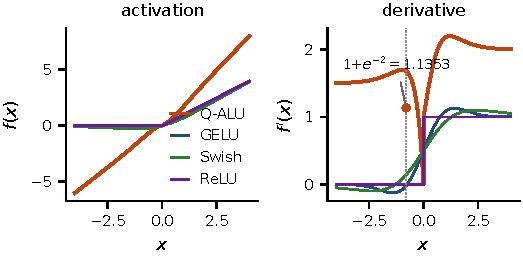
\includegraphics[width=\columnwidth]{figures/activation.pdf}
\caption{Left: the four activations. Right: their derivatives. Q-ALU's negative
branch peaks at $1.1353\gamma$ at $x=-2\delta$ (dotted), a $13.53\%$ overshoot;
its positive branch peaks $9.98\%$ above the $2\alpha$ asymptote.}
\label{fig:act}
\end{figure}

\begin{figure*}[t]
\centering
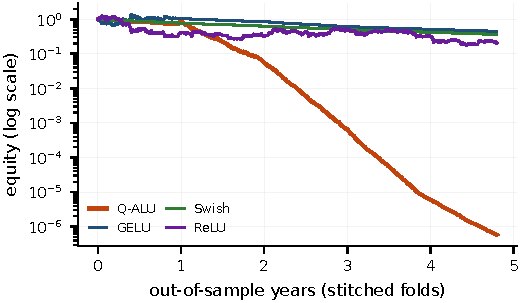
\includegraphics[width=\textwidth]{figures/equity.pdf}
\caption{Stitched out-of-sample equity curves of the four candidates over the
five walk-forward test blocks (log scale). The curves are the equal-weight
ensemble of \nSeeds{} paired seeds.}
\label{fig:equity}
\end{figure*}

\resultText

\section{Discussion}

\paragraph{What the experiment can and cannot say}
The sample is one instrument on one venue, and the models are deliberately
small: the entire grid is trained on a single commodity CPU. A four-way
comparison at this scale can detect a large effect and cannot detect a small
one; the paired confidence intervals in Table~\ref{tab:results} are the honest
statement of what the data supports, and a null result here is evidence about
this protocol, not a proof that activations are irrelevant in general.

\paragraph{Why the cost term matters}
With a 5\,bp fee, a policy that changes position every bar pays
$5\,\mathrm{bp}\times 10^5\approx50\%$ of notional per year before any
forecast, which exceeds the annualised volatility of most intraday signals. The
turnover column of Table~\ref{tab:results} is therefore not a secondary
diagnostic: any activation that produces a jumpier policy is penalised twice,
once in the objective and once in the reported Sharpe.

\paragraph{Training stability}
The budget a single commodity CPU allows is small, and the Differential-Sharpe
objective is a ratio of two noisy batch statistics. Across the grid,
\spreadSentence{}. Two failure modes appear: the policy collapses to a
near-constant long position, or it chatters and pays the fee on almost every
bar. Which one a run lands in is decided early in training and is visible in the
turnover column long before it is visible in the Sharpe. Reporting the mean over
paired seeds without that spread would overstate the precision of the comparison.

\paragraph{Deployment}
The exported model is a pure feed-forward computation: a grouped convolution
with a $T$-tap kernel, element-wise recurrence coefficients folded at export
time, and two small linear maps. The ONNX artifact is \onnxKb\,KB. TorchScript
and ONNX Runtime outputs agree with PyTorch to within \parity{} in maximum
absolute deviation. On the reference machine (Intel Celeron N2930, no AVX)
single-bar inference takes \latencyTorch\,ms (p50) under TorchScript and
\latencyOnnx\,ms (p50) under ONNX Runtime, and the incremental resident set of an
isolated inference process is \rssOnnx\,MB, inside the 50\,MB budget. The budget
holds because no term in the model is quadratic in $T$: the convolution is
$O(T k D)$ and the recurrence is $O(T D N)$ with $N=8$.

\section{Conclusion}

We built a causal, attention-free dual-stream state-space policy, gave an exact
calculus for its Q-ALU core, and compared four activations under a
pre-registered purged walk-forward protocol with paired seeds and three
independent statistical tests. \conclusionSentence{} The code, the split
definitions, the per-cell artifacts and the exported models are released so
that the claim can be checked rather than trusted.

\balance
\begin{thebibliography}{00}
\bibitem{qalu} F.~H.~Mutaqin, ``Q-ALU: Quant Asymmetric Leaky Unit,''
Cyclocerine Research Initiative, 2026. SSRN 7365098.
\bibitem{s4} A.~Gu, K.~Goel, and C.~R\'e, ``Efficiently modeling long sequences
with structured state spaces,'' in \emph{Proc. ICLR}, 2022.
\bibitem{mamba} A.~Gu and T.~Dao, ``Mamba: Linear-time sequence modeling with
selective state spaces,'' \emph{arXiv:2312.00752}, 2023.
\bibitem{relu} V.~Nair and G.~E.~Hinton, ``Rectified linear units improve
restricted Boltzmann machines,'' in \emph{Proc. ICML}, 2010.
\bibitem{gelu} D.~Hendrycks and K.~Gimpel, ``Gaussian error linear units
(GELUs),'' \emph{arXiv:1606.08415}, 2016.
\bibitem{swish} P.~Ramachandran, B.~Zoph, and Q.~V.~Le, ``Searching for
activation functions,'' \emph{arXiv:1710.05941}, 2017.
\bibitem{purgedcv} M.~L\'opez de Prado, \emph{Advances in Financial Machine
Learning}. Wiley, 2018.
\bibitem{dm} F.~X.~Diebold and R.~S.~Mariano, ``Comparing predictive accuracy,''
\emph{J. Bus. Econ. Stat.}, vol.~13, no.~3, pp.~253--263, 1995.
\bibitem{nw} W.~K.~Newey and K.~D.~West, ``A simple, positive semi-definite,
heteroskedasticity and autocorrelation consistent covariance matrix,''
\emph{Econometrica}, vol.~55, no.~3, pp.~703--708, 1987.
\bibitem{politis} D.~N.~Politis and J.~P.~Romano, ``The stationary bootstrap,''
\emph{J. Amer. Statist. Assoc.}, vol.~89, no.~428, pp.~1303--1313, 1994.
\bibitem{dsr} D.~H.~Bailey and M.~L\'opez de Prado, ``The deflated Sharpe ratio:
correcting for selection bias, backtest overfitting, and non-normality,''
\emph{J. Portfolio Manage.}, vol.~40, no.~5, pp.~94--107, 2014.
\bibitem{psr} D.~H.~Bailey and M.~L\'opez de Prado, ``The Sharpe ratio efficient
frontier,'' \emph{J. Risk}, vol.~15, no.~2, pp.~3--44, 2012.
\bibitem{moody} J.~Moody and M.~Saffell, ``Learning to trade via direct
reinforcement,'' \emph{IEEE Trans. Neural Netw.}, vol.~12, no.~4, pp.~875--889,
2001.
\end{thebibliography}

\end{document}
